\documentclass{article}
\usepackage{indentfirst}
\usepackage{ctex}
\usepackage{geometry}
\usepackage{graphicx, subfigure}
\usepackage{enumerate}
\geometry{left=3.17cm,right=3.17cm,top=2.54cm,bottom=2.54cm} % 页边距

\begin{document}

\title{Google File System}
\date{}
\maketitle

\begin{abstract}
我们设计并实现了Google File System,这是为大规模分布式数据密集型应用程序打造的一个可扩展(scalable)的分布式文件系统。虽然GFS运行在廉价的日用硬件上,但它仍然提供了容错功能,并且为大量客户端提供了总体上的高性能。\par
虽然GFS与之前的分布式文件系统有着很多相同的目标,但是,我们的设计已受到了当前和可预计的将来的应用工作负载和技术环境的驱使,这也反映出GFS和早期分布式文件系统的明显差距。这也驱使我们重新审视传统分布式文件系统的技术选择,探索极为不同的设计要点。\par
GFS成功地满足了我们的存储需求。GFS作为存储平台,被广泛部署在Google内部,用于数据的生成与处理,这些数据用于我们的各类服务中,以及研究和开发工作中所需的大规模数据集。迄今为止,最大的集群通过数千台机器上的数千磁盘提供了数百TB的存储服务,为数以百计的客户端所访问。\par
本文中,我们将展示用以支持分布式应用的文件系统接口扩展,并讨论设计的方方面面,最后给出小规模基准测试和真实使用环境下的测试结果。
\end{abstract}

\section{INTRODUCTION}
(第一段内容基本和摘要一致)\par
第一,组件故障是常态(norm)而非异常。文件系统由成百上千的存储机器组成,而这些机器是使用廉价的日用部件组装而成的;其次,有相当数量的客户端访问会访问文件系统。由于组件的大数量和低质量,几乎任何时刻都会有一些组件失效,并且无法从当前故障中恢复。我们遇到过各种BUG,有的来自应用程序,有的来自操作系统,有的来自人为错误,以及磁盘、内存、网络甚至是电源供给的故障。因此,持续的监控,错误检测,容错,以及自动恢复功能必须集成到系统中。\par
第二,以传统标准衡量,GFS的文件非常巨大,数GB的很常见。每个文件通常包含许多应用对象,比如web文档。当我们经常处理快速增长的数TB的数据集——这些数据集由数百万对象组成——的时候,将难以管理数百万的KB级的小文件,即使文件系统是支持的。这样一来,就必须重新考虑设计思路和参数设置,比如I/O操作和块数据大小。\par
第三,对大多数文件的修改是通过追加数据而不是覆盖已有数据,也不存在对文件的随机写。文件一经写入就成为只读的,而且通常只允许顺序读。各种类型的数据都遵循这一特性,这些数据中,有的构成了数据分析程序扫描的巨大数据仓库,有的是运行中的应用程序持续生成的数据流,有的是归档数据,有的是在一台机器上产生并在另一台机器上处理过程中生成的中间数据。有了这种针对大文件的访问模式,追加操作只需关注性能优化和原子性保证,而并不关注数据块的缓存。\par
第四,通过提高整个系统的灵活性,我们可以应用和文件系统API的协同设计从中受益。例如,我们降低了对GFS一致性模型的要求,在不给应用施加繁重负担的条件下极大地简化了文件系统设计。我们还引入了一种原子追加操作,使得多个客户端能够并发地向一个文件追加数据,而无需额外的同步。这些内容将在下文中详细讨论。\par
当前出于不同目的,我们部署了多个GFS集群。最大的一个拥有1000多个存储节点,300多TB的磁盘存储,并且承受着来自不同机器数以百计的持续访问。

\section{DESIGN OVERVIEW(设计概要)}
\subsection{Assumptions}
在设计符合我们需求的文件系统时,我们的假设一直都是挑战与机遇并存的。我们之前曾提到过一些值得注意的关注点,现在我们将从更多的细节出发,进一步阐释我们的假设。
\begin{itemize}
	\item 用于组装系统的组件都是日用的廉价产品,它们经常出故障,所以必须持续监控自身状态,周期性地查错、容错,并且能够迅速从故障中恢复。
	\item 系统存储了一定数量的大文件,文件数量估计在几百万,每个文件大约100MB或更大。GB级的大文件很常见,需要得到高效处理;同时必须能够支持小文件,但我们需要一些优化工作。
	\item 工作负载主要来自两种类型的读操作:大规模流式读和小规模随机读。对于大规模流式读,单次读取的数据量通常有数百KB,比较常见的则是1MB或者更大。来自同一客户端的一系列读操作通常读取的是一个文件中的连续区域。对于小规模随机读,通常会从文件中的任意偏移地址开始,读取几KB的数据。对性能要求较高的应用一般把小规模的读操作进行排序和批处理,如此一来,读操作变得更加平稳。
	\item 工作负载亦可来自向文件追加数据时的大规模序列化写操作。通常,写操作的数据量与读操作较为接近。文件一经写入便不再修改。在文件中任意偏移地址上的小规模写虽然是允许的,但这会降低系统效率。
	\item 系统必须为多个并发地向同一文件追加数据的客户端定义明确的语义。我们的文件经常被用于“生产者-消费者”队列和多路合并之中。数百个消费者,每个运行在一台机器上,并发地向同一个文件追加数据——在这种情况下,如何以最小的同步开销实现原子性就显得至关重要。文件可能稍后被读取,或者消费者在追加数据的同时读取文件。
	\item 可持续的高带宽比低延迟更重要。大多数应用看重的是高速地处理大块数据,而对单一的读写操作没有严格的相应时间要求。
\end{itemize}

\subsection{Interface}
GFS提供了一套常见的文件系统接口,但是它未实现类似于POSIX的标准API。文件以目录树的形式分层组织,以路径名进行标识。我们提供了文件的以下几种常规操作:\emph{create},\emph{delete},\emph{open},\emph{close},\emph{read},\emph{write}。\par
另外,GFS提供了\emph{shapshot}和\emph{record append}操作。shapshot能够以低廉的开销创建一个文件或目录的拷贝。record append允许多个客户端并发地向同一个文件追加数据,同时能够保证每个客户端操作的原子性。这有助于实现多路合并和“生产者-消费者”队列,无需对多个客户端的追加操作添加额外的锁。我们发现这些类型的文件对于构建大型分布式应用非常有价值。 我们将在后文中分别讨论shapshot和record append。

\subsection{Architecture}
如图\ref{fig:GFS_Arch}所示,GFS集群由一个\emph{master}和多个\emph{chunkservers}构成,被多个客户端访问。集群中的每个组件通常是一个运行用户级服务进程的Linux机器。只要机器上的资源允许,并且由于行为古怪的应用程序代码所导致的低可靠性是可接受的,我们就很容易在同一机器上同时运行chunkserver和client。\par
\begin{figure}[htbp]
    \centering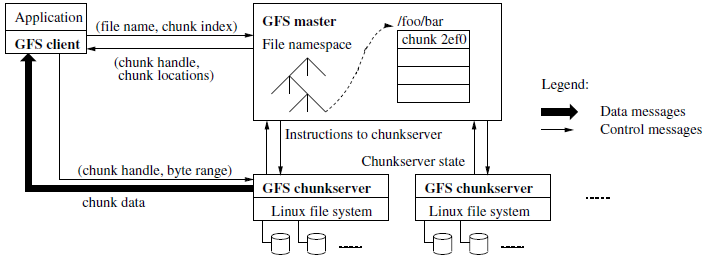
\includegraphics[height=5cm]{images/GFS_Arch.png}
    \caption{GFS Architecture}
    \label{fig:GFS_Arch}
\end{figure}
文件被分割成大小固定的\emph{chunks}。每个chunk由一个不可修改的64bit全局\emph{chunk handle}标识——master在创建chunk的时候对chunk handle赋值。为了保证可靠性,每个chunk都在多个chunkservers上存有副本。缺省设置下,我们保存3个副本,但是用户可以为文件命名空间中的不同区域指定不同的赋值级别。\par
master维护所有文件系统元数据——包括命名空间,访问控制信息,文件到chunks的映射关系,chunks的当前位置。master还控制着整个系统的活动,比如chunk租约管理,孤儿chunks的垃圾回收,chunk在chunkservers之间的迁移。master通过心跳(\emph{HeartBeat})消息周期性地与每个chunkserver通信,向其发送指令并收集其状态信息。\par
链接到每个应用程序中的GFS客户端代码的功能是:实现文件系统API;与master和chunkservers通信,替应用程序读写数据。客户端和master交互元数据操作,但是所有承载数据的(data-bearing)的通信都是与chunkservers直接进行的。我们不提供POSIX API,因此不需要在Linux的vnode层设置钩子。\par
客户端和chunkserver均不对文件数据进行缓存。客户端缓存收效甚微,因为大多数应用要么对大文件进行流式处理,要么因为工作集太大而无法缓存。因为没有了缓存,也就不存在缓存一致性问题,使客户端和整个系统的设计得到简化(但是客户端会缓存元数据)。chunkservers无需缓存文件数据,因为chunks是以本地文件的形式进行存储,所以Linux的缓冲区缓存技术已经把经常被访问的数据缓存在内存中了。

\subsection{Single Master}
只设置一个单独的master极大地简化了我们的设计,让master能够使用全局信息完成复杂的chunk部署和副本决策。然而,我们必须最小化其中的读写相关性,不至于让其成为系统瓶颈。客户端永远不会通过master读写文件数据。相反,客户端通询问master它应该连接到哪一个chunkserver。客户端将该信息缓存一定时间,并直接和chunkservers交互来完成后续的操作。\par
我们参照图\ref{fig:GFS_Arch}来解释一个简单的读操作涉及的交互过程。首先,客户端按照固定的chunk大小将文件名和应用程序指定的字节偏移转换为文件中的chunk索引。然后,客户端向master发送一个请求,请求中包含文件名和chunk索引。master把chunk句柄(handle)和chunk副本的位置回复给客户端。客户端以文件名和chunk索引作为key,将该信息添加到缓存中。客户端之后会向其中一个副本发送请求,一般是距离最近的那个。请求中指定了chunk句柄和chunk的字节范围。之后对同一个chunk的读操作就不再需要client-master之间的交互,直到缓存过期或者文件被重新打开。事实上,客户端通常在一个请求中请求多个chunks,master亦可立即包含请求中的chunks的信息。这些额外的信息回避了client-master之间未来的交互——这么做实际上并没有额外的开销。

\subsection{Chunk Size}
chunk的尺寸是设计参数中的一个要点。我们选择64MB,这远大于常规文件系统中的块大小。每一个chunk副本在chunkserver上保存为一个普通的Linux文件,只有在需要的时候进行扩展。懒惰空间分配避免了内部碎片(internal fragmentation)导致的空间浪费,而这可能是对于如此巨大的chunk尺寸的最有争议的地方。\par
巨大的chunk尺寸具有若干重要的优势。第一,减少了客户端和master之间的交互次数,因为对同一个chunk的读写只需要和master的一次初始请求即可获得chunk的位置信息。这种削减对于工作负载的降低很有意义,因为应用经常对大文件进行顺序读写。即使对于小规模随机读,客户端也能为一个数TB工作集缓存其中的chunk位置信息。第二,因为采用大尺寸的chunk,客户端容易在一个给定的chunk上执行许多操作,通过在长时间(over an extended period of time)内维持与chunkserver的持久TCP连接,可以减轻网络负载。第三,减小了存储在master上的元数据的大小,有助于将元数据驻留在内存中,这也带来了其他优势。\par
另一方面,即使配合懒惰空间分配,大尺寸chunk依然存在缺陷。一个小文件也许只由一个或极少数量的chunks组成。如果许多客户端访问同一个文件,存储这些chunks的chunkservers可能变成热点(hot spots)。在实际应用中,热点并非主要问题,因为我们的应用多数情况下只会对包含多个chunk的大文件进行顺序读。\par
然而,当GFS第一次被批处理队列系统使用的时候,热点问题还是显露了:一个可执行程序作为一个单独的chunk文件被写入GFS,之后在数百台机器上同时启动。保存这个可执行程序的几个chunkservers被数百个并发请求造成过载。我们以更高的复制因子来存储这样的可执行程序,并且让批处理队列系统错开(stagger)应用的启动时间,如此才解决了这一问题。一种可能的(potential)长期解决方案是:在该情形下,允许客户端从其他客户端读取数据(译者注:类似于p2p)。

\subsection{Metadata}
master存储3中主要类型的元数据:文件和chunk的命名空间,文件到chunk的映射关系,每一个chunk副本的位置信息。所有元数据都驻留在master的内存中。前两种元数据(namespaces and file-to-chunk mapping)为了持久化,还会将修改日志记录到存储在master本地磁盘上的操作日志(operation log)中,同时在远程机器上留有副本。使用日志允许我们能够简单可靠地更新master的状态,当master崩溃的时候不至于冒数据不一致的风险。master不会持久保存chunk位置信息。相反,master在启动时以及新chunkserver加入集群时,向各个chunkserver询问它们的chunks信息。

\subsubsection{In-Memory Data Structures}
由于元数据存储在内存中,所以master的数据操作很快。此外,master更容易在后台 高效地周期性扫描自身的整个状态。这种周期性扫描被用于实现chunk的垃圾回收,chunkserver宕机时的chunk重复制,以及chunk迁移(chunk迁移用于均衡跨chunkservers的负载和磁盘空间使用)。\par
这种memory-only方式的一个潜在问题在于chunks的数量,而且整个系统的容量受限于master所拥有的内存大小。在实际中,这并不是一个严格的限制。master为每一个64MB的chunk所维护的元数据不超过64bytes。大多数chunks都被占满,因为大多数文件包含很多chunks,只有随后一个可能只填充了一部分。类似地,每个文件的命名空间数据量通常不超过64bytes,因为文件名是使用前缀压缩方式压缩存储的。\par
如果有必要支持更大的文件系统,相对于将元数据存储在master的内存中所获得的简单性、可靠性、性能和灵活性,为master扩充内存的开销是很小的。

\subsubsection{Chunk Locations}
master不会持久保存“哪个chunkserver持有给定的chunk副本”的记录,它只是在启动之时简单地轮询chunkservers以获得该信息,此后master通过周期性的心跳消息掌控所有chunk的部署,并监控chunkserver的状态,因此master能够保持自身状态的持续更新。\par
我们最初试图把master上的chunk位置信息进行持久化,但我们发现,让master在启动时从chunkservers上请求这些数据、之后周期性地轮询会更容易。这么做消除了在chunkservers加入/离开集群、更名、故障、重启的时候,保持master和chunkservers同步的问题。在一个拥有数百服务器的集群中,这些事件经常发生。\par
理解这一设计的另一种方式是认识到只有chunkserver能决定chunks是否存在于它的磁盘上。试图在master上维持该信息的一致视图(consistent view)是毫无意义的,因为chunkserver上的错误可能造成chunks自发消失(比如磁盘故障),或者操作人员可能对一个chunkserver重命名。

\subsubsection{Operation Log}
操作日志包含关键元数据变更的历史记录,对于GFS很重要。操作日志不仅是元数据的唯一持久化记录,而且作为逻辑时间定义了并发操作的顺序。文件和chunks,以及它们的版本,均由它们被创建时的逻辑时间唯一、永久地标识。\par
因为操作日志极为重要,所以需要被可靠地存储,只有元数据的更改被持久化后,才能使其(指元数据的更改)对客户端可见。否则,即使chunks自身存活了下来,我们也要有效地丢失整个文件系统或最近的客户端操作(译者注:这句话是什么意思?)。因此,我们需要把操作日志拷贝到多台远程机器上,并且只有等到客户端把相应的日志记录刷写到本地和远程机器的磁盘上之后,才响应客户端操作。master在刷盘之前,对多条日志记录进行批处理,因此可以降低刷盘和复制对整个系统吞吐量的影响。\par
master通过回放操作日志来恢复自身文件系统状态。为了最小化系统的启动时间,我们必须让日志尽量的小。每当日志增长至一定大小时,master就对自身状态做一次检查点,如此一来,master就能够通过从本地磁盘中加载最近的检查点,并回放其后(最近的检查点之后)一定数量的日志记录,来进行系统恢复。检查点是一个紧密的类B-tree的结构,可以被直接映射到内存,并且无需额外的解析即可被用于命名空间的查询,显著加速了系统恢复速度,提高了可用性。\par
由于创建检查点需要一定时间,所以master的内部状态被以这样的方式组织:能够在不阻塞后续修改操作的同时创建一个新的检查点。master在一个单独的线程中切换到新的日志文件,并创建新的检查点。新的检查点包括本次切换前的所有修改记录。对于一个拥有数百万文件的集群,检查点能够在几分钟内创建完成。创建完成后,它将被写入本地和远程机器的磁盘中。\par
系统恢复只需最近一次做完的检查点,及该检查点之后的日志文件。较旧的检查点和日志文件可以随意删除,但是我们会保存一部分以应对灾难性故障(catastrophes)。创建检查点期间出现的故障不会影响其正确性,因为用以实现系统恢复的代码会检测到故障,并跳过为完成的检查点。

\subsection{Consistency Model(一致性模型)}
GFS有一个宽松的一致性模型,对我们高度分布的应用提供了很好的支持,相对简单也易于高效地实现。我们现在讨论GFS为应用提供的一致性保障和意义,也会强调GFS如何维护这种保障,至于细节方面则留给其他章节。

\subsubsection{Gurantees by GFS}
文件命名空间的的修改(比如创建文件)是原子性的。它们由master互斥地处理:命名空间锁保证了原子性和正确性;master的操作日志(operation log)定义了这些操作的全局完整顺序。\par
数据变更后的文件域(file region)状态取决于修改的类型、成功与否、是否存在并发修改。如果文件域能够在文件数据修改后保证一致性,那么这个文件域就是“已定义的(defined)”,并且客户端会看到修改时写入的全部内容。在不干涉并发写者的前提下完成对文件数据的修改后,受影响的文件域就变成“已定义的”(暗含了一致性):所有客户端总是会看到修改时写入的内容。并发的修改成功后,文件域处于“未定义”、一致的状态:所有客户端看到的是相同的数据,但并不能反映出任意一个修改操作写入的内容。失败的修改让文件域处于不一致状态(因此也是未定义的):不同的客户端可能在不同时刻看到不同的数据。我们将在下文中描述我们的应用如何区分已定义和未定义的文件域。应用不需要进一步区分不同类型的未定义文件域。\par
数据的修改可能来自\emph{writes}或\emph{record appends}。写操作:将数据写入文件中应用程序制定的偏移地址处。记录追加操作:即使面临并发修改,也能将数据(记录)原子性地追加至少一次,但是是在GFS选定的偏移上。(相比之下,一次常规的追加操作仅仅是在某个偏移地址上的写操作——这个偏移在应用程序看来就是当前文件末尾。)这个GFS选定的偏移被返回给客户端,用于标记包含记录的、已定义的文件域的开始。另外,GFS可能在中间插入填充数据或重复记录——这些内容占据了被认定为不一致的文件域,其大小相比于用户数据通常微不足道。\par
在一系列成功的修改操作之后,被修改的文件域一定是已定义的,并且包含了最后一次修改所写入的数据。GFS实现这一特性的方法是:(a)对某个chunk的所有副本以相同的顺序应用修改,(b)使用chunk版本号来检测过时的(stale)副本——这些过时的副本在管理它们的chunkserver 宕机的时候就丢失了修改。过时的副本不会涉及修改操作,也不会被提供给向master查询chunk位置的客户端。系统将尽快对其进行垃圾回收。\par
因为客户端缓存了chunk的位置信息,所以它们可能在信息被刷新之前,就从过时的副本中读取数据。这个窗口受限于缓存项的超时时间和下一次文件打开操作——这会清除该文件在缓存中所有chunk的信息。另外,因为大多数文件是append-only的,所以从过时的副本中通常会返回一个提前结束的chunk,而非过期数据。当reader重新尝试连接master时,它会立即获得当前chunk的位置信息。\par
在一次成功的修改操作的很长时间后,组件故障仍然会破坏数据。GFS通过master和所有chunkservers之间周期性的握手来识别失效的chunkservers,并通过计算校验和的方式来检测出数据的损坏。一旦问题出现,数据就从有效的副本中尽快得到恢复。只有某个chunk的所有副本在GFS做出反应之(GFS的反应时间通常在数分钟内)全部丢失,这个chunk的丢失才是不可逆转的。即使在这种情况下,chunk也只是变为不可用的,而不会被损坏:应用会接收到清晰的错误信息,而不是损坏的数据。

\subsubsection{Implications for Applications}
GFS应用只需一些简单的技术即可适应宽松的一致性模型,这些技术已经满足了其他目的需要:依赖于追加写而不是覆盖写,检查点,写操作的自校验,记录的自标识。\par
实际中,所有的应用程序都是通过追加而不是覆盖的方式修改文件。一个典型的例子是,writer按照从头到尾的顺序生成一个文件。完成所有数据的写入之后,writer原子性地将文件重命名为一个永久的名字,或者周期性地创建检查点,记录成功写入的数据量。检查点可能包括应用程序级别的校验和。readers只校验并处理上一个检查点之前的文件域——已知该文件域处于已定义状态。抛开一致性和并发性不谈,这种方法很适合我们。追加写相比于随机写具有更高的效率,也更不容易受应用程序故障的影响。检查点允许writers增量式重启,防止readers处理成功写入的文件数据——这些文件数据在应用程序看来仍然是不完整的。\par
在另一种典型场景中,多个writers为了合并结构或者作为“生产者-消费者”队列,并发地向一个文件追加数据。记录追加操作的“至少追加一次”的语义保留了每个writer的输出结果。readers对偶尔的填充数据和重复记录进行处理。writer准备好的每一条记录都包含额外的信息,比如校验和,使得数据的有效性得到校验。reader能通过校验和识别出额外的填充数据和记录片段,并将其丢弃。如果reader不能容忍偶尔的重复记录(例如,这些重复记录会触发非幂等操作),就可以使用记录中唯一的标识符将其过滤掉,这些标识符也被用于命名相应的应用程序实体,比如web文档。这些I/O记录功能(除了移除重复数据)被封装为应用程序的共享代码库,并被用于Google的其他文件接口的实现。这样一来,相同的记录序列,加上些许的重复记录,总是被分发到读取记录的reader。

\section{SYSTEM INTERACTIONS(系统交互)}
我们设计这个系统力图最小化master在所有操作中的参与度。在此背景下,我们现在描述客户端,master,以及chunkservers如何交互,如何实现数据修改、原子性记录追加和快照。

\subsection{Leases and Mutation Order}
修改操作指的是对chunk的内容或元数据的修改,比如写入和追加操作。每个修改操作都在所有的chunk副本上执行。我们使用租约来维持副本间的一致性修改顺序。master将一个chunk租约授予该chunk的一个副本,我们把这个副本叫做主副本(\emph{primary})。主副本为chunk的所有修改操作选择一个顺序。所有副本在应用修改的时候都遵照这一顺序。于是,全局修改顺序首先由master选定的租约授予顺序定义,然后在租约内部由主副本分配的序号定义。\par
设计租约机制是为了最小化master的管理负载。租约的初始超时时间为60s。然而,只要chunk正在被修改,主副本向master发出请求后通常会受到无限期的租约延长。这些租约延长请求和授予信息搭载在master与chunkservers之间的周期性心跳消息之上。master有时可能会试图在租约到期之前撤销之(比如,当master想禁止对一个正在被重命名的文件的修改)。即使master失去了和主副本的通信,它也可以在旧租约到期后,安全地向另一个副本授予一个新的租约。
\begin{figure}[htbp]
    \centering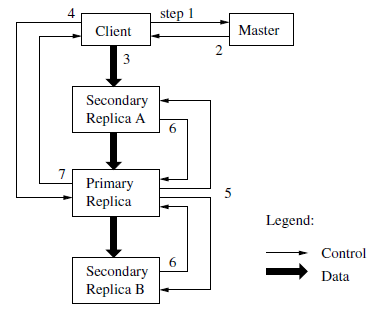
\includegraphics[height=5cm]{images/write_control_and_data_flow.png}
    \caption{Write Control and Data Flow}
    \label{fig:write_control_and_data_flow}
\end{figure}
在图\ref{fig:write_control_and_data_flow}中,我们根据写操作的控制流按照这些标号步骤阐述了这一过程。
\begin{enumerate}
	\item 客户端询问master哪一个chunkserver持有chunk的当前租约,以及其他chunk副本的位置。如果没有chunkserver持有租约,master将租约授予它选择的chunk副本(未在途中展示)。
	\item master将主副本的标识信息和其他(secondary,次级)副本的位置信息回复给客户端。客户端将这些数据缓存下来,用于未来的修改操作。客户端只有在主副本不可达,或者回复不再持有租约时,才需要再次连接master。
	\item 客户端将数据推送到所有副本。客户端可以以任意顺序完成推送。每个chunkserver将数据存储在内部的LRU缓存中,直到数据被使用或者过期。通过数据流和控制流的解耦,我们可以基于网络拓扑调度昂贵的数据流,而不必关心哪一个chunkserver持有主副本,以此提高系统性能。
	\item 一旦所有副本确认接收到了数据,客户端就会像主副本发送一个写请求。该请求标识了之前推动给所有副本的数据。主副本为它接受到的所有修改分配连续的序号,由于修改可能来自多个客户端,这就提供了必要的序列化。主副本按照序号顺序将修改应用到自己的本地状态。
	\item 主副本将写请求转发(forward)到所有次级副本。每一个次级副本按照主副本分配的序号以相同的顺序应用修改。
	\item 所有次级副本回复主副本,表明他们已经完成了操作。
	\item 次级副本回复客户端。任何副本遇到的任何错误都被报告给客户端。在出错的情况下,在主副本和次级副本的任意子集上的写操作可能已经成功完成。(如果写操作在主副本上失败,主副本就不会分配序号和转发请求。)客户端请求被认定为失败,已修改的文件域处于不一致状态。我们的客户端代码处理该错误的方法是:重试失败的修改。在退回到写操作的开头进行重试之前,客户端会在step(3)到(7)之间做一些尝试。
\end{enumerate}
\par
如果应用程序的一次写入量过大或者跨越了chunk边界,GFS客户端代码就将这一次写操作分裂为多个写操作。它们都遵循上面描述的控制流,但是可能和来自其他客户端的并发操作交织在一起,并被其覆盖。因此,共享文件域最终可能会包含来自不同客户端的片段,但是由于这些单独的操作在所有副本上都以相同的顺序成功完成,所以副本都是相同的。这会让文件域处于一致但未定义的状态,如Section 2.7中所述。

\end{document}